
\section{recall: window size versus bandwidth}
\usetikzlibrary{arrows.meta,calc}

\begin{frame}[fragile,label=throughAndWindow]{throughput and window size}
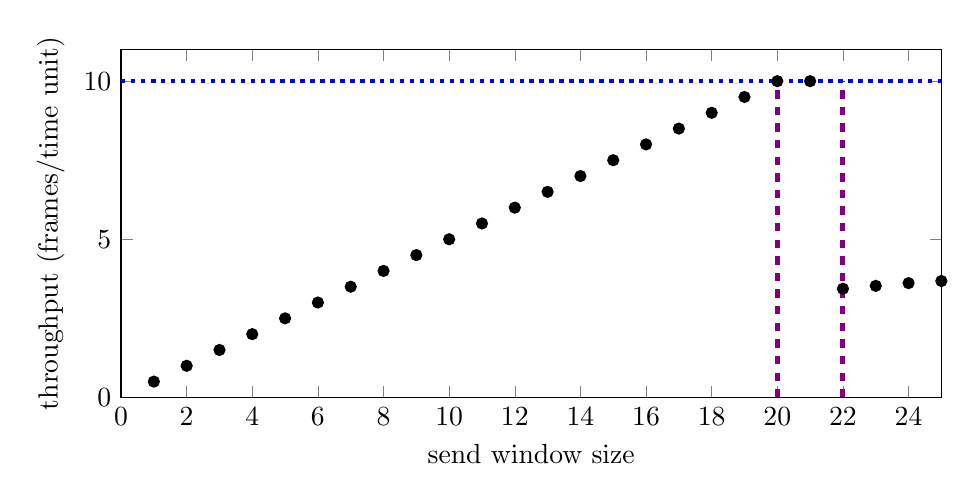
\begin{tikzpicture}
\begin{axis}[width=12cm,height=6cm,
    xlabel=send window size,
    ylabel=throughput (frames/time unit),
    xmin=0,xmax=25,ymin=0]
\addplot[only marks] coordinates {
(1, 0.5000025000125)
(2, 1.0000090000810007)
(3, 1.4999925000374998)
(4, 2.0000280003920055)
(5, 2.500037500562508)
(6, 3.000003000003)
(7, 3.5000035000035)
(8, 4.000048000576006)
(9, 4.499842505512307)
(10, 5.000025000125)
(11, 5.499975250111374)
(12, 5.99977200866367)
(13, 6.499710762871052)
(14, 6.999811005102861)
(15, 7.4996812635462975)
(16, 7.999680012799485)
(17, 8.499426288725509)
(18, 8.999361045365776)
(19, 9.499202067026369)
(20, 9.999100080971061)
(21, 9.999100080973866)
(22, 3.435635094325549)
(23, 3.5274986154570636)
(24, 3.613708966335035)
(25, 3.6808686850100703)
(26, 3.753260645186032)
(27, 3.8487443471573166)
(28, 3.925956461143474)
};
\addplot[blue,dotted,ultra thick,domain=0:25] {10};
    \draw[violet,dashed,ultra thick] (axis cs:20,0) -- (axis cs:20, 10)
     coordinate (empty queue mark);
    \draw[violet,dashed,ultra thick] (axis cs:21.99,0) -- (axis cs:21.99, 10)
     coordinate (full queue mark);
\end{axis}
\end{tikzpicture}
\end{frame}

\usetikzlibrary{arrows.meta,calc}

\begin{frame}{simple network model}
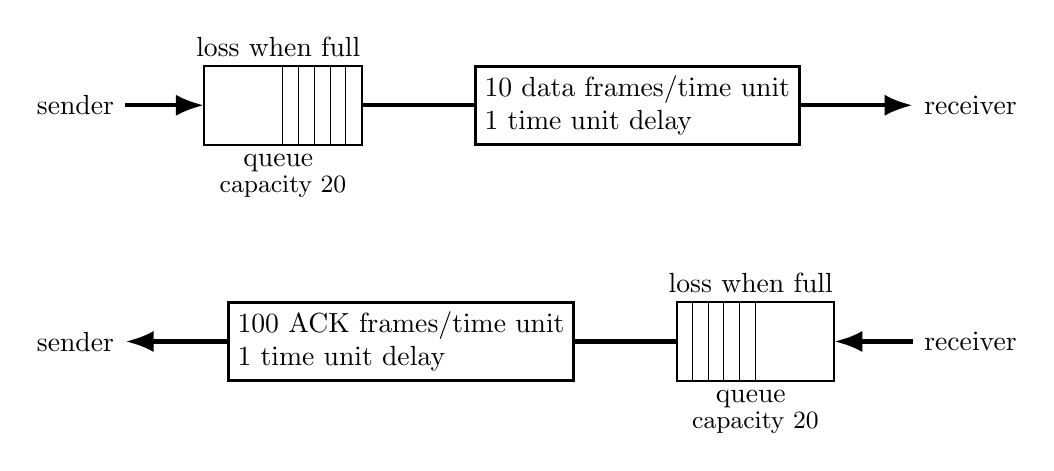
\begin{tikzpicture}
\draw[ultra thick,arrows={-Latex}] (0, 0) node[left] {sender} -- (1, 0);
\draw[thick] (1, -.5) rectangle (3, .5);
\foreach \x in {2,2.2,2.4,2.6,2.8} {
    \draw (\x, -.5) -- (\x, .5);
}
\node[anchor=south,align=center] at (2, .5) {
    loss when full
};
\node[anchor=north,align=center] at (2, -.5) (queue label) {
    queue
};
\node[anchor=north,font=\small] at ([yshift=.2cm]queue label.south) {
    capacity 20
};
\draw[ultra thick,arrows={-Latex}] (3, 0) -- (10, 0) node[right]{receiver}
    node[midway,fill=white,draw=black,very thick,align=left] {
        10 data frames/time unit \\
        1 time unit delay
    };
\begin{scope}[shift={(10, -3)},x=-1cm]
    \draw[ultra thick,arrows={-Latex}] (0, 0) node[right] {receiver} -- (1, 0);
    \draw[thick] (1, -.5) rectangle (3, .5);
    \foreach \x in {2,2.2,2.4,2.6,2.8} {
        \draw (\x, -.5) -- (\x, .5);
    }
    \node[anchor=south,align=center] at (2, .5) {
        loss when full
    };
    \node[anchor=north,align=center] at (2, -.5) (queue label) {
        queue
    };
    \node[anchor=north,font=\small] at ([yshift=.2cm]queue label.south) {
        capacity 20
    };
    \draw[ultra thick,arrows={-Latex}] (3, 0) -- (10, 0) node[left]{sender}
        node[midway,fill=white,draw=black,very thick,align=left] {
            100 ACK frames/time unit \\
            1 time unit delay
        };
\end{scope}
\end{tikzpicture}
\begin{itemize}
\item simulator from upcoming assignment
    \begin{itemize}
    \item command line \texttt{--delay 1 --bandwidth-forward 10 --bandwidth-backward 100 --buffer 30}
    \end{itemize}
\end{itemize}
\end{frame}

\begin{frame}{exercise: forward latency}
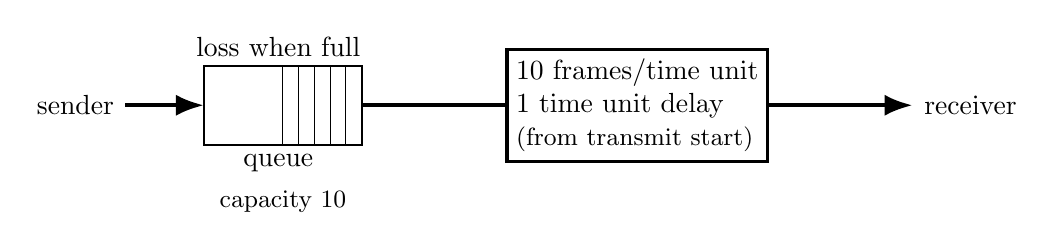
\begin{tikzpicture}
\draw[ultra thick,arrows={-Latex}] (0, 0) node[left] {sender} -- (1, 0);
\draw[thick] (1, -.5) rectangle (3, .5);
\foreach \x in {2,2.2,2.4,2.6,2.8} {
    \draw (\x, -.5) -- (\x, .5);
}
\node[anchor=south,align=center] at (2, .5) {
    loss when full
};
\node[anchor=north,align=center] at (2, -.5) (queue label) {
    queue
};
\node[anchor=north,font=\small] at (queue label.south) {
    capacity 10
};
\draw[ultra thick,arrows={-Latex}] (3, 0) -- (10, 0) node[right]{receiver}
    node[midway,fill=white,draw=black,very thick,align=left] {
        10 frames/time unit \\
        1 time unit delay \\
        \small (from transmit start)
    };
\end{tikzpicture}
\begin{itemize}
\item minimum latency = 1 time unit
\item exercise: maximum latency?
\end{itemize}
\begin{tabular}{lll}
A. 1 time unit & B. 1.1 time unit & C. 1.2 time unit \\
C. 1.4 time unit & D. 1.9 time unit & E. 2.0 time unit \\
F. 2.1 time unit & G. something else \\
\end{tabular}
\end{frame}

\begin{frame}[fragile,label=throughAndWindow]{throughput and window size}
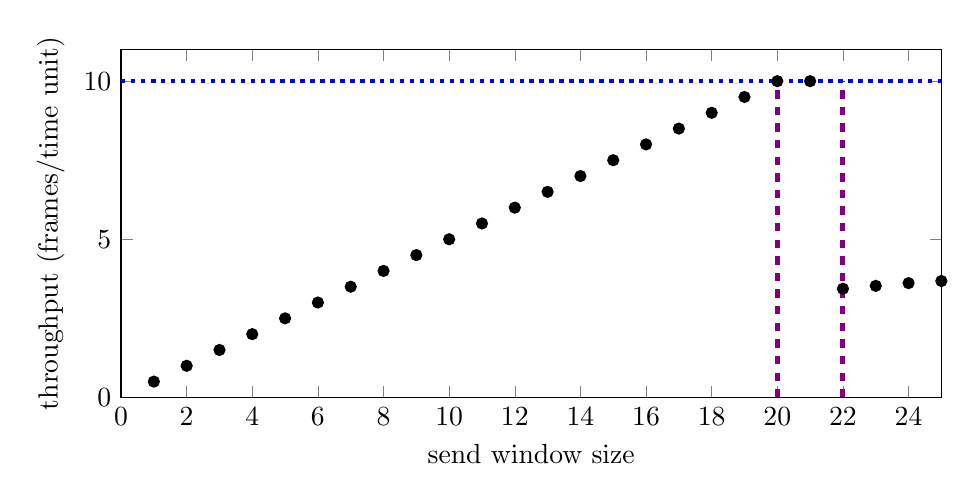
\begin{tikzpicture}
\begin{axis}[width=12cm,height=6cm,
    xlabel=send window size,
    ylabel=throughput (frames/time unit),
    xmin=0,xmax=25,ymin=0]
\addplot[only marks] coordinates {
(1, 0.5000025000125)
(2, 1.0000090000810007)
(3, 1.4999925000374998)
(4, 2.0000280003920055)
(5, 2.500037500562508)
(6, 3.000003000003)
(7, 3.5000035000035)
(8, 4.000048000576006)
(9, 4.499842505512307)
(10, 5.000025000125)
(11, 5.499975250111374)
(12, 5.99977200866367)
(13, 6.499710762871052)
(14, 6.999811005102861)
(15, 7.4996812635462975)
(16, 7.999680012799485)
(17, 8.499426288725509)
(18, 8.999361045365776)
(19, 9.499202067026369)
(20, 9.999100080971061)
(21, 9.999100080973866)
(22, 3.435635094325549)
(23, 3.5274986154570636)
(24, 3.613708966335035)
(25, 3.6808686850100703)
(26, 3.753260645186032)
(27, 3.8487443471573166)
(28, 3.925956461143474)
};
\addplot[blue,dotted,ultra thick,domain=0:25] {10};
    \draw[violet,dashed,ultra thick] (axis cs:20,0) -- (axis cs:20, 10)
     coordinate (empty queue mark);
    \draw[violet,dashed,ultra thick] (axis cs:21.99,0) -- (axis cs:21.99, 10)
     coordinate (full queue mark);
\end{axis}
\end{tikzpicture}
\end{frame}

\begin{frame}[fragile,label=transitTime]{packet transit time}
\begin{tikzpicture}
\draw[ultra thick,arrows={-Latex}] (0, 0) node[left] {sender} -- (1, 0);
\draw[thick] (1, -.5) rectangle (3, .5);
\foreach \x in {2,2.2,2.4,2.6,2.8} {
    \draw (\x, -.5) -- (\x, .5);
}
\node[anchor=south,align=center] at (2, .5) {
    loss when full
};
\node[anchor=north,align=center] at (2, -.5) (queue label) {
    queue
};
\node[anchor=north,font=\fontsize{9}{10}\selectfont] at ([yshift=.3cm]queue label.south) {
    capacity 20
};
\draw[ultra thick,arrows={-Latex}] (3, 0) -- (12, 0) node[right]{receiver}
    node[midway,fill=white,draw=black,very thick,align=left] {
        10 data frames/time unit \\
        1 time unit delay
    }
    node[visible on=<1-3>,ultra thick,pos=0,draw=black,fill=white,font=\tiny,below=.5cm] (data-main) {data};
    \begin{visibleenv}<2->
    \draw[red,-Latex,very thick] (data-main.east) -- (data-main.west -| 13, 0) coordinate (end send)
        node[midway,below,font=\small] {1 time unit (sender to receiver)};
    \end{visibleenv}
\begin{scope}[shift={(12, -4)},x=-1cm]
    \draw[ultra thick,arrows={-Latex}] (0, 0) node[right] {receiver} -- (1, 0);
    \draw[thick] (1, -.5) rectangle (3, .5);
    \foreach \x in {2,2.2,2.4,2.6,2.8} {
        \draw (\x, -.5) -- (\x, .5);
    }
    \node[anchor=south,align=center] at (2, .5) {
        loss when full
    };
    \node[anchor=north,align=center] at (2, -.5) (queue label) {
        queue
    };
    \node[anchor=north,font=\small] at ([yshift=.2cm]queue label.south) {
        capacity 20
    };
    \draw[ultra thick,arrows={-Latex}] (3, 0) -- (12, 0) node[left]{sender}
        node[midway,fill=white,draw=black,very thick,align=left] {
            100 ACK frames/time unit \\
            1 time unit delay
        }
        node[visible on=<2->,pos=0,draw=red,fill=white,font=\tiny,below=.5cm,align=center,inner sep=0.5mm] 
            (ack-start) {a\\c\\k};
    \begin{visibleenv}<2->
        \draw[dotted,red,-Latex,very thick] (end send) |- (ack-start.east);
        \draw[red,-Latex,very thick] (ack-start.west) -- (ack-start.west -| 12, 0) node[midway,below,font=\small] { + 1 time unit (receiver to sender)};
    \end{visibleenv}
\end{scope}
\begin{visibleenv}<3>
\node[draw=red,fill=white,ultra thick,align=left] at (6, -2.5) {
    takes 1 + 1 time units to send message + receive ack \\
    goal: keep sending stuff while waiting
};
\end{visibleenv}
\end{tikzpicture}
\end{frame}

\begin{frame}{filling the pipe}
    \begin{itemize}
    \item round-trip time of 2 time units
        \begin{itemize}
        \item from send data to receive ACK (assuming no queuing delay)
        \end{itemize}
    \item can send 10 data frames per time unit
    \item = can send 20 data frames while waiting for ACK
    \vspace{.5cm}
    \item<2> \myemph{``bandwidth-delay product''}
        \begin{itemize}
        \item 10/time unit (banwidth) times 2 time unit (RTT = delay)
        \end{itemize}
    \end{itemize}
\end{frame}

\begin{frame}[fragile,label=throughAndWindow]{throughput and window size (detail)}
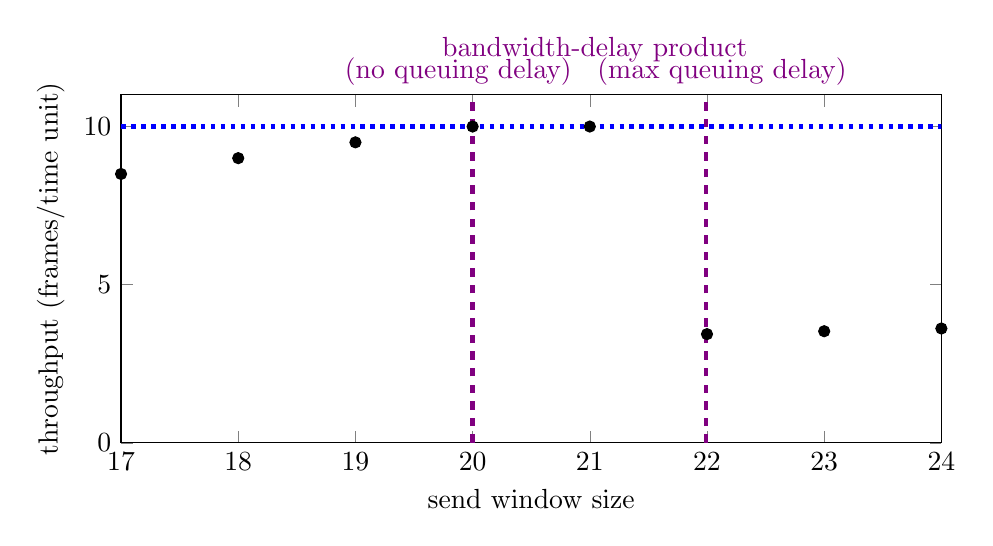
\begin{tikzpicture}
\begin{axis}[width=12cm,height=6cm,
    xlabel=send window size,
    ylabel=throughput (frames/time unit),
    xmin=17,xmax=24,ymin=0]
\addplot[only marks] coordinates {
(1, 0.5000025000125)
(2, 1.0000090000810007)
(3, 1.4999925000374998)
(4, 2.0000280003920055)
(5, 2.500037500562508)
(6, 3.000003000003)
(7, 3.5000035000035)
(8, 4.000048000576006)
(9, 4.499842505512307)
(10, 5.000025000125)
(11, 5.499975250111374)
(12, 5.99977200866367)
(13, 6.499710762871052)
(14, 6.999811005102861)
(15, 7.4996812635462975)
(16, 7.999680012799485)
(17, 8.499426288725509)
(18, 8.999361045365776)
(19, 9.499202067026369)
(20, 9.999100080971061)
(21, 9.999100080973866)
(22, 3.435635094325549)
(23, 3.5274986154570636)
(24, 3.613708966335035)
(25, 3.6808686850100703)
(26, 3.753260645186032)
(27, 3.8487443471573166)
(28, 3.925956461143474)
};
\addplot[blue,dotted,ultra thick,domain=0:25] {10};
    \draw[violet,dashed,ultra thick] (axis cs:20,0) -- (axis cs:20, 11)
     coordinate (empty queue mark);
    \draw[violet,dashed,ultra thick] (axis cs:21.99,0) -- (axis cs:21.99, 11)
     coordinate (full queue mark);
\end{axis}
\node[violet,anchor=south east,align=right] (nq) at ([xshift=1.5cm]empty queue mark) {
    (no queuing delay)
};
\node[violet,anchor=south west,align=left] (mq) at ([xshift=-1.5cm]full queue mark) {
    (max queuing delay)
};
\node[violet,anchor=south] at ($(nq)!0.5!(mq)$) {bandwidth-delay product};
\end{tikzpicture}
\end{frame}


\begin{frame}[fragile,label=fullPipe]{filling the pipe}
\begin{tikzpicture}
\draw[ultra thick,arrows={-Latex}] (0, 0) node[left] {sender} -- (1, 0);
\draw[thick] (1, -.5) rectangle (3, .5);
\foreach \x in {2,2.2,2.4,2.6,2.8} {
    \draw (\x, -.5) -- (\x, .5);
}
\node[anchor=south,align=center] at (2, .5) {
    loss when full
};
\node[anchor=north,align=center] at (2, -.5) (queue label) {
    queue
};
\node[anchor=north,font=\fontsize{9}{10}\selectfont] at ([yshift=.3cm]queue label.south) {
    capacity 20
};
\draw[ultra thick,arrows={-Latex}] (3, 0) -- (12, 0) node[right]{receiver}
    node[midway,fill=white,draw=black,very thick,align=left] {
        10 data frames/time unit \\
        1 time unit delay
    }
    \foreach \x in {0,1,2,3,4,5,6,7,8,9} {
        node[visible on=<3->,pos=\x*.1+0.05,draw=black,fill=white,font=\tiny,below=.5cm] (data-\x) {data}
    };
    \begin{visibleenv}<3->
    \draw[red,Latex-Latex] ([yshift=-.1cm]data-0.south west) -- ([yshift=-.1cm]data-1.south west)
        node[below,font=\small] {0.1 time unit};
    \end{visibleenv}
\begin{scope}[shift={(12, -4)},x=-1cm]
    \draw[ultra thick,arrows={-Latex}] (0, 0) node[right] {receiver} -- (1, 0);
    \draw[thick] (1, -.5) rectangle (3, .5);
    \foreach \x in {2,2.2,2.4,2.6,2.8} {
        \draw (\x, -.5) -- (\x, .5);
    }
    \node[anchor=south,align=center] at (2, .5) {
        loss when full
    };
    \node[anchor=north,align=center] at (2, -.5) (queue label) {
        queue
    };
    \node[anchor=north,font=\small] at ([yshift=.2cm]queue label.south) {
        capacity 20
    };
    \draw[ultra thick,arrows={-Latex}] (3, 0) -- (12, 0) node[left]{sender}
        node[midway,fill=white,draw=black,very thick,align=left] {
            100 ACK frames/time unit \\
            1 time unit delay
        }
        \foreach \x in {0,1,2,3,4,5,6,7,8,9} {
            node[visible on=<3->,pos=\x*.1+0.05,draw=black,fill=white,font=\tiny,below=.5cm,align=center,inner sep=0.5mm] {a\\c\\k}
        };
\end{scope}
\end{tikzpicture}
\end{frame}


\section{why optimal / counting packets in flight}
\begin{frame}{why optimal}
    \begin{itemize}
    \item in normal operation with window size $W$
        \begin{itemize}
        \item receive ACK for $x$ (now $W-1$ in flight)
        \item send packet $x+W$
        \item receive ACK for $x+1$
        \item send packet $x+W+1$
        \item \ldots
        \end{itemize}
    \item window size keeps $W$ packets in flight
    \item if links + queues can hold $W$ packets --- perfect!
    \end{itemize}
\end{frame}

\begin{frame}{number in flight on losses}
    \begin{itemize}
    \item window size $W$
    \item let's say we lose packet $x$ [only], sender might
        \begin{itemize}
        \item receive ACK for $x-1$
        \item send packet $x+W-1$
        \item receive ACK for $x$, $x$, $x$, \ldots
        \item resend packet $x$ (guess it is lost)
        \item \myemph<2>{receive ACK for $x$, $x$, $x$, \ldots}
        \item receive ACK for packet $x+W-1$ 
        \item send packets $x+W$ through $x+W+W-1$
        \end{itemize}
    \end{itemize}
\begin{tikzpicture}[overlay,remember picture]
\begin{visibleenv}<2->
\node[draw=red,ultra thick,anchor=south,align=left] at ([yshift=1cm]current page.south) {
    lots of time where we are not sending packets \\
    means network is underutilized
};
\end{visibleenv}
\end{tikzpicture}
\end{frame}

\begin{frame}{window size tweaking}
    \begin{itemize}
    \item window size imperfect proxy for \# packets in flight
    \item we'll ignore the difference for now
    \vspace{.5cm}
    \item our goal for now: window size = number of packets to have in flight
    \end{itemize}
\end{frame}



\section{searching for performance}
\usetikzlibrary{arrows.meta,shapes.misc,shapes.geometric}
\begin{frame}{finding window size empirically (1)}
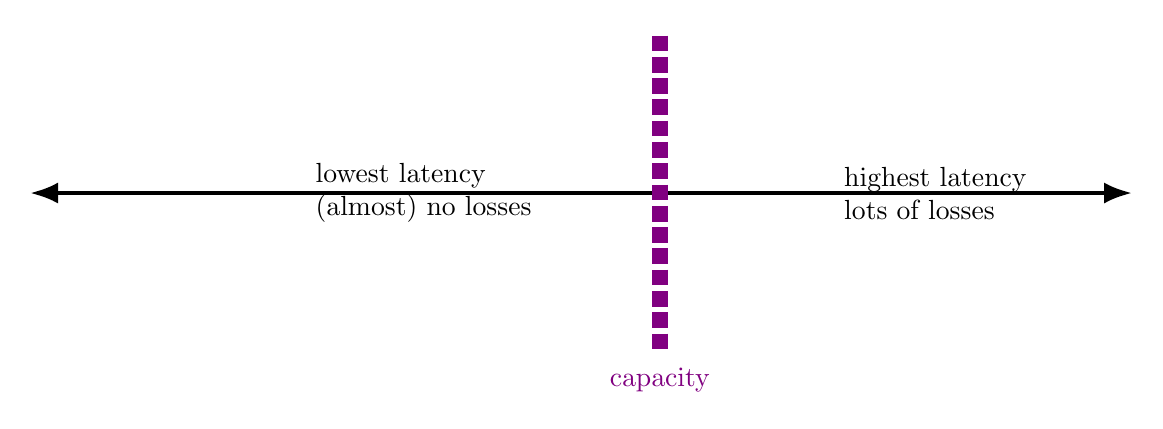
\begin{tikzpicture}
\draw[ultra thick,Latex-Latex] (-7, 0) -- (7, 0);
\draw[dotted,line width=2mm,violet] (1, 2) -- (1, -2) node[below] {capacity};
\node[align=left] at (-2, 0) {
    lowest latency \\
    (almost) no losses
};
\node[align=left] at (4.5, 0) {
    highest latency \\
    lots of losses 
};
\end{tikzpicture}
\end{frame}

\begin{frame}{key insight}
    \begin{itemize}
    \item latency/loss rate increases when window size too big
    \item latency/loss rate stable when window size not too big
    \vspace{.5cm}
    \item for now, we'll focus on loss rate
        \begin{itemize}
        \item but you can do something similar with latency
        \end{itemize}
    \end{tiemize}
\end{frame}

\begin{frame}{try a bunch of things}
\begin{tikzpicture}
\tikzset{
    good/.style={draw,star,thick,fill=green!70!black},
    bad/.style={draw,cross out,red!70!black,line width=3mm},
}
\draw[ultra thick,Latex-Latex] (-7, 0) -- (7, 0);
\node at (0, -.5) {window size};
\node[good,label={east:= low loss rate}] (key good) at (-6, 2) {};
\node[bad,label={east:= high loss rate}] (key bad) at (-6, 1) {};
\begin{visibleenv}<2->
\node[good] at (-3, 0){};
\node[bad] (high bad) at (5, 0){};
\end{visibleenv}
\begin{visibleenv}<3->
\node[bad] at (1, 0){}; 
\end{visibleenv}
\begin{visibleenv}<4->
\node[good] at (-1, 0){}; 
\end{visibleenv}
\begin{visibleenv}<5->
\node[good] at (-0.5, 0){}; 
\node[good] at (-0.2, 0){}; 
\node[bad] at (0.3, 0){}; 
\node[bad] at (0.5, 0){}; 
\node[bad] at (0.9, 0){}; 
\end{visibleenv}
\begin{visibleenv}<6>
\draw[Latex-,very thick] (high bad) -- ++(-2, -5) node {
    what is the network like when we do this?
};
\end{visibleenv}
\end{tikzpicture}
\end{frame}


\section{a little history}
\begin{frame}{revisiting congestion collapse}
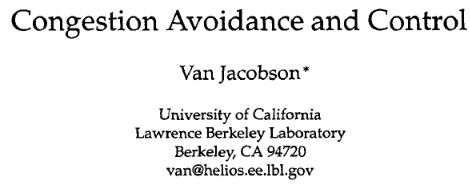
\includegraphics[width=0.6\textwidth]{../congest/jacobson-title}
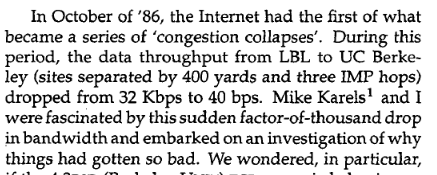
\includegraphics[width=0.6\textwidth]{../congest/jacobson-disaster}
\end{frame}

\begin{frame}<1>[label=jacobsonFixes]{fixes from Jacobson's 1987 paper}
\begin{tikzpicture}
\node[anchor=north west] (fixes) at (0, 0) {
    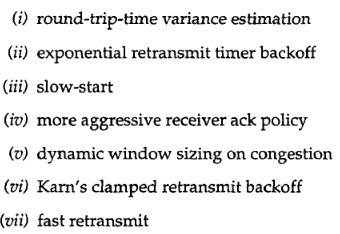
\includegraphics[width=0.6\textwidth]{../congest/jacobson-fixes}
};
%\path[draw,help lines] (0, 0) grid[step=1] (8, -5);
\begin{visibleenv}<2>
    \draw[red,ultra thick] (0, -3.8) rectangle (9, -4.4);
\end{visibleenv}
\begin{visibleenv}<4>
    \draw[red,ultra thick] (0, -2) rectangle (3, -2.8);
\end{visibleenv}
\begin{visibleenv}<3>
    \draw[red,ultra thick] (0, -5.4) rectangle (4.5, -6.2);
\end{visibleenv}
\end{tikzpicture}
\end{frame}


% FIXME: up/down pattern with constant bandwidth available [from CUBIC?]
    % FIXME: use to ask question why do we keep trying to increase window?

% FIXME: preview actual window size graphs in simulation
\section{performance collapse}
\begin{frame}{the overloaded switch}
\begin{itemize}
\item let's say switch can handle 50 packets/second
\item but has:
    \begin{itemize}
    \item 100 packets/second from test flow sending as fast as it can
    \item 10 packets/second from other session
    \end{itemize}
\item expected \textit{loss rate} (\% packets lost)?
\item expected \% test flow packets lost?
\item expected other session packets lost?
\end{itemize}
\end{frame}

\begin{frame}{modeling who gets dropped}
    \begin{itemize}
    \item it kinda does matter\ldots
    \item sending in big bursts or spread out (``pacing'')?
        \begin{itemize}
        \item bursts can overload queues even though average rate is low
        \end{itemize}
    \item how switch's queue works?
        \begin{itemize}
        \item queue size (handling bursts), way to choose what to drop
        \end{itemize}
    \item random or fixed intervals between sending?
    \vspace{.5cm}
    \item<2-> but we'll \myemph<2>{simplify}, assuming---
        \begin{itemize}
        \item a flow's arrivals are randomly spaced
        \item drops hit packets at random
        \item queue is ``pretty big''
        \end{itemize}
    \end{itemize}
\end{frame}

\begin{frame}{the overloaded switch}
\begin{itemize}
\item let's say switch can handle 50 packets/second
\item but has:
    \begin{itemize}
    \item 100 packets/second from test flow (checking window size) 
    \item 10 packets/second from other session
    \end{itemize}
\item expected \textit{loss rate} (\% packets lost)? $\frac{100+10-50}{100+10}=54\%$
\item expected \% test flow packets lost? $54\%$
\item expected \% other session packets lost? $54\%$
\item<2-> \myemph{\ldots but I missed something}
\end{itemize}
\end{frame}

\begin{frame}{a virtuous cycle}
\begin{itemize}
\item what is other session going to when 54\% of its packets are lost?
    \begin{itemize}
    \item probably resend them
    \end{itemize}
\item what about when resent packets are lost?
    \begin{itemize}
    \item probably resent again
    \end{itemize}
\vspace{.5cm}
\item if other session doesn't slow down, then\ldots
\item $10$ pkt/s $\rightarrow10+54\%\cdot10+54\%^2\cdot10 \ldots\approx 22$ pkt/s
\end{itemize}
\end{frame}


\begin{frame}{the overloaded switch (revised)}
\begin{itemize}
\item let's say switch can handle 50 packets/second
\item but has:
    \begin{itemize}
    \item 100 packets/second from test flow (checking window size) 
    \item 10 packets/second from other session $\rightarrow 22$ with resends
    \end{itemize}
\item expected \textit{loss rate} (\% packets lost)? $\frac{100+22-50}{100+22}=59\%$
\item expected \% test flow packets lost? $59\%$
\item expected \% other session packets lost? $59\%$
    \begin{itemize}
    \item<2-> means that 22 pkt/sec is slight underestimate
    \item<2-> though realistically other session should slow down
    \end{itemize}
\end{itemize}
\end{frame}

\begin{frame}{aside: latency (1)}
\begin{itemize}
\item 589% packet loss $\rightarrow$ average packet sent 2.4 times
\item need one round-trip time (RTT) to detect loss
    \begin{itemize}
    \item probably from duplicate ACK
    \item if detecting via timeout, probably longer
    \end{itemize}
\item so need 1.4 RTTs (detecting loss 1.4 times) extra time 
\item mean latency $= \frac{1.4 \text{RTTs}}{0.5 \text{RTTs}}$ times normal $= 2.8$ times normal
\end{itemize}
\end{frame}

\begin{frame}{aside: high-percentile latency}
\begin{itemize}
\item 59\% packet loss
\item about 10\% of time need more than 4 retransmissions
\item about 5\% of the time need more than 5 retransmissions
\item about 1\% of the time need more than 8 retransmissions
\end{itemize}
\end{frame}

\begin{frame}{sliding windows and retransmissions}
    \begin{itemize}
    \item assuming that other session doesn't slow down
    \vspace{.5cm}
    \item sliding window approach slows down on losses
    \end{itemize}
\end{frame}

\begin{frame}{sliding window throughput collapse}
\begin{itemize}
\item let's say doing sliding window with 100 packet window
\item if 1\% of the time, we need to resend a packet 8 times, then
\item probably need around 8 RTTs to send all 100 packets in window
\vspace{.5cm}
\item<2-> $\approx$ 8 times slower with same window size
\end{itemize}
\end{frame}


\section{heuristic: slow increase}
\begin{frame}{slow increase}
    \begin{itemize}
    \item want to increase \textit{slowly} to avoid overload
    \item original TCP: +1 packet/round trip time
    \vspace{.5cm}
    \item<2-> +1 certainly not optimal choice, but okay heuristic
    \item<2-> important theoretically: approx. \myemph{additive} increase
        \begin{itemize}
        \item helps ensure good behavior with multiple connections
        \item (we'll talk later about why)
        \end{itemize}
    \end{itemize}
\end{frame}


\subsection{exercise: convergence times}
\begin{frame}{exercise: convergence time (1)}
    \begin{itemize}
    \item suppose: 50 ms round trip time
    \item initially sending at 600 packets/second
        \begin{itemize}
        \item $\approx 0.9$Mbyte/sec with 1500 byte packets
        \end{itemize}
    \item optimal rate is 10000 packets/second
        \begin{itemize}
        \item $\approx 15$Mbyte/sec with 1500 byte packets
        \end{itemize}
    \item `standard' TCP increase of 1 packet/RTT
    \item how long to get there?
    \item<2-> current: 30 packets/RTT (= window size 30)
    \item<2-> need to get to: 500 packets/RTT
    \item<2-> will take $500-30=470$ round trips $\approx$ 23500 ms $\approx$ 24 s
    \end{itemize}
\end{frame}

\begin{frame}{fixing bad convergence time}
    \begin{itemize}
    \item TCP's additive increase is very slow for ``high bandwidth-delay'' networks
    \item two things make this better:
    \vspace{.5cm}
    \item not in additive increase mode at start of connection
        \begin{itemize}
        \item ``slow start'' we'll talk about later
        \end{itemize}
    \item more adaptive increase for modern TCP variants
        \begin{itemize}
        \item e.g. FAST TCP, CUBIC TCP, \ldots
        \item heuristics to increase faster when appropriate
        \end{itemize}
    \end{itemize}
\end{frame}


% FIXME: no slow start example versus real

\section{changing cross-traffic}

\usetikzlibrary{arrows.meta,calc,shapes}
\providecommand{\computer}{%
    
\includegraphics[width=1cm]{../common/Noun_project_216.pdf}
}
\providecommand{\switch}{%
    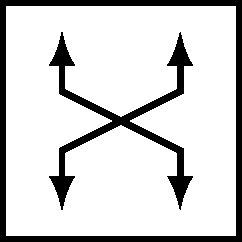
\includegraphics[width=0.9cm]{../common/fig-switch.pdf}
}
\providecommand{\router}{%
    
\includegraphics[width=0.9cm]{../common/fig-router.pdf}
}



\begin{frame}{changing cross-traffic}
\begin{tikzpicture}
\tikzset{
    computer/.style={inner sep=0mm,outer sep=0mm,execute at begin node={\computer}},
    switch/.style={inner sep=0mm,outer sep=0mm,execute at begin node={\switch}},
    router/.style={inner sep=0mm,outer sep=0mm,execute at begin node={\router},circle},
    connect/.style={draw,very thick,Latex-Latex},
    connect big/.style={draw,ultra thick,Latex-Latex},
}
\node[computer] (A) at (0, 0){};
\node[computer] (B) at (13, 0){};
\node[router] (r1) at (5, 0){};
\node[router] (r2) at (10, 0){};
\node[computer] (C) at (3, 3){};
\node[computer] (D) at (12, -3){};
\foreach \x/\y in {A/r1,r1/r2,r2/B,C/r1,r2/D} {
    \draw[connect] (\x) -- (\y);
}
\begin{visibleenv}<2>
\foreach \x/\y in {A/r1,r1/r2,r2/B} {
    \draw[blue,line width=1mm] ([yshift=-1mm]\x) -- ([yshift=-1mm]\y);
}
\node[text=blue,anchor=north] at ([yshift=-3mm]$(A)!0.5!(r1)$) {10Mbit};
\end{visibleenv}
\begin{visibleenv}<3>
\foreach \x/\y in {A.east/r1.west,r1.east/r2.west,r2.east/B.west} {
    \draw[-Latex,blue,line width=1mm] ([yshift=-3mm]\x) -- ([yshift=-3mm]\y);
}
\foreach \x/\y in {C/r1,r1.east/r2.west,r2/D} {
    \draw[-Latex,red,dotted,line width=1mm] ([yshift=3mm]\x) -- ([yshift=3mm]\y);
}
\node[text=blue,anchor=north] at ([yshift=-3mm]$(A)!0.5!(r1)$) {\sout{10Mbit} 7Mbit};
\node[text=red,anchor=west] at ($(C)!0.5!(r1)$) {3Mbit};
\end{visibleenv}
\begin{visibleenv}<4>
\foreach \x/\y in {A/r1,r1/r2,r2/B} {
    \draw[blue,line width=1mm] ([yshift=-1mm]\x) -- ([yshift=-1mm]\y);
}
\node[text=blue,anchor=north] at ([yshift=-3mm]$(A)!0.5!(r1)$) {\sout{10Mbit} \sout{7Mbit} 10Mbit};
\end{visibleenv}
\end{tikzpicture}
\end{frame}

\begin{frame}{adapting to cross-traffic}
    \begin{itemize}
    \item available bandwidth will change
    \item previous example: 3Mbit lost/added from other flow
    \vspace{.5cm}
    \item need to adapt to lost bandwidth
    \item need to detect new available bandwidth
    \end{itemize}
\end{frame}

\begin{frame}{other flow's bandwidth?}
    \begin{itemize}
    \item for now, we'll pretend other flows don't react to us
    \vspace{.5cm}
    \item later topic: what happens when both reacting?
    \end{itemize}
\end{frame}



\section{up/down pattern (rough)}
\begin{frame}{window size experimenting}
\begin{tikzpicture}
\tikzset{
    axis line/.style={draw,line width=1mm,-Latex},
    optimum/.style={draw,line width=0.5mm,dashed},
    actual/.style={draw,line width=0.75mm,violet,line to},
    down segment/.style={},
}
    \begin{scope}[y=.8cm,x=.9cm]
        \path[fill=red!10] (0, 6) rectangle (6, 8);
        \path[fill=red!10] (6, 4) rectangle (10, 8);
        \path[fill=red!10] (10, 6) rectangle (14, 8);
        \node[text=red!70!black] at (8, 7) {packets dropped sometimes};
        \node[text=green!70!black] at (8, 2) {packets not dropped};
        
        \path[actual]
            (0, 5.5) to
            (3, 6.3) coordinate (down1) to
            (3, 5.5) to
            (4, 5.8) to
            (6.1, 6.1) coordinate (down2) to
            (6.1, 5.7) to
            (6.5, 5.9) coordinate (down3) to
            (6.5, 5.5) to
            (6.7, 5.7) coordinate (down4) to
            (6.7, 4.8) to
            (6.8, 4.9) coordinate (down5) to
            (6.8, 3.7) to
            (7, 3.8) to
            (8, 4.2) coordinate (down6) to
            (8, 3.5) to
            (9, 3.7) to 
            (10, 4.1) to
            (11, 5.7) to
            (12.5, 6.2) coordinate (down7) to
            (12.5, 5.7) to
            (13, 5.8) to 
            (14, 6.1);

        \foreach \x in {1,...,7} {
            \node[draw=red,cross out,line width=2mm] at (down\x) {};
        };

        \path[axis line] (0, 0) -- (0, 8);
        \path[axis line] (0, 0) -- (14, 0);
        \node[anchor=north] at (7, 0) {time};
        \node[anchor=east,align=center] at (0, 4) {window\\size};
        \path[optimum] (0, 6) -- (6, 6);
        \path[optimum] (6, 4) -- (10, 4);
        \path[optimum] (10, 6) -- (14, 6);
        \begin{visibleenv}<2>
            \node[draw=red,fill=white,ultra thick,align=left,overlay,anchor=north] (up msg) at (3, 2) {
                always try increasing window size
            };
        \end{visibleenv}

        \begin{visibleenv}<3>
            \node[draw=red,fill=white,ultra thick,align=left,overlay,anchor=north] (drop msg) at (3, 2) {
                react to drops \\ by decreasing window
            };
            \foreach \x in {1,...,7} {
                \path[draw=red!50!black, very thick,-Latex] (drop msg) -- (down\x);
            }
        \end{visibleenv}
    \end{scope}
\end{tikzpicture}
\end{frame}

\begin{frame}{increase/decrease strategy}
    \begin{itemize}
    \item default to increasing window size
    \item react to packet drops by decreasing window size
        \begin{itemize}
        \item \myemph<2>{assumption: few ``non-congestion'' packet losses}
        \end{itemize}
    \vspace{.5cm}
    \item<3-> big topic: how fast to do each?
    \item<3-> questions to help decide that:
        \begin{itemize}
        \item what happens if we increase too fast? too slow?
        \item what happens if we decrease too fast? too slow?
        \end{itemize}
    \end{itemize}
\end{frame}

    % FIXME: show sawtooth pattern

\section{heuristic: fast decrease (v1)}
\begin{frame}{heurstic: fast decrease (v1)}
    \begin{itemize}
    \item want to decrease quickly to get out of overload
    \item original TCP heuristic: reset window to 1 packet
    \end{itemize}
\end{frame}


\section{heuristic: fast decrease (v2)}
\begin{frame}{fast decrease}
    \begin{itemize}
    \item want to decrease quickly to get out of overload
    \item original TCP heuristic: divide by two (minimum 1 packet)
    \vspace{.5cm}
    \item<2-> exactly by two probably not important
    \item<2-> important theoretically: approx. \myemph{multiplicative} decrease
        \begin{itemize}
        \item will help show okay behavior with multiple flows
        \end{itemize}
    \end{itemize}
\end{frame}

\begin{frame}{AIMD}
    \begin{itemize}
    \item additive increase + multiplicative decrease
    \item basic of steady-state behavior
    \end{itemize}
\end{frame}


\section{AIMD}

\begin{frame}{AIMD}
    \begin{itemize}
    \item result: additive increase + multiplicative decrease
    \vspace{.5cm}
    \item preview: good theoretical properties for \textit{sharing connections}
        \begin{itemize}
        \item doesn't matter much what additive/multiplicative factor is!
        \end{itemize}
    \item but: not quite what current Internet does
    \end{itemize}
\end{frame}


\section{part 1: window sizing}
\againframe<2>{jacobsonFixes}

\section{focus on steady state}
\begin{frame}{handling steady state}
    \begin{itemize}
    \item most of the time we should be at approx. correct window size
    \vspace{.5cm}
    \item want to focus on how we react to changes
    \item still going to use ``experimentation'' idea
    \end{itemize}
\end{frame}

    % FIXME: hilite distance measurement oof down parts on sawtooth pattern

\section{some graphs}
\begin{frame}[label=vegasrenotrace]{}
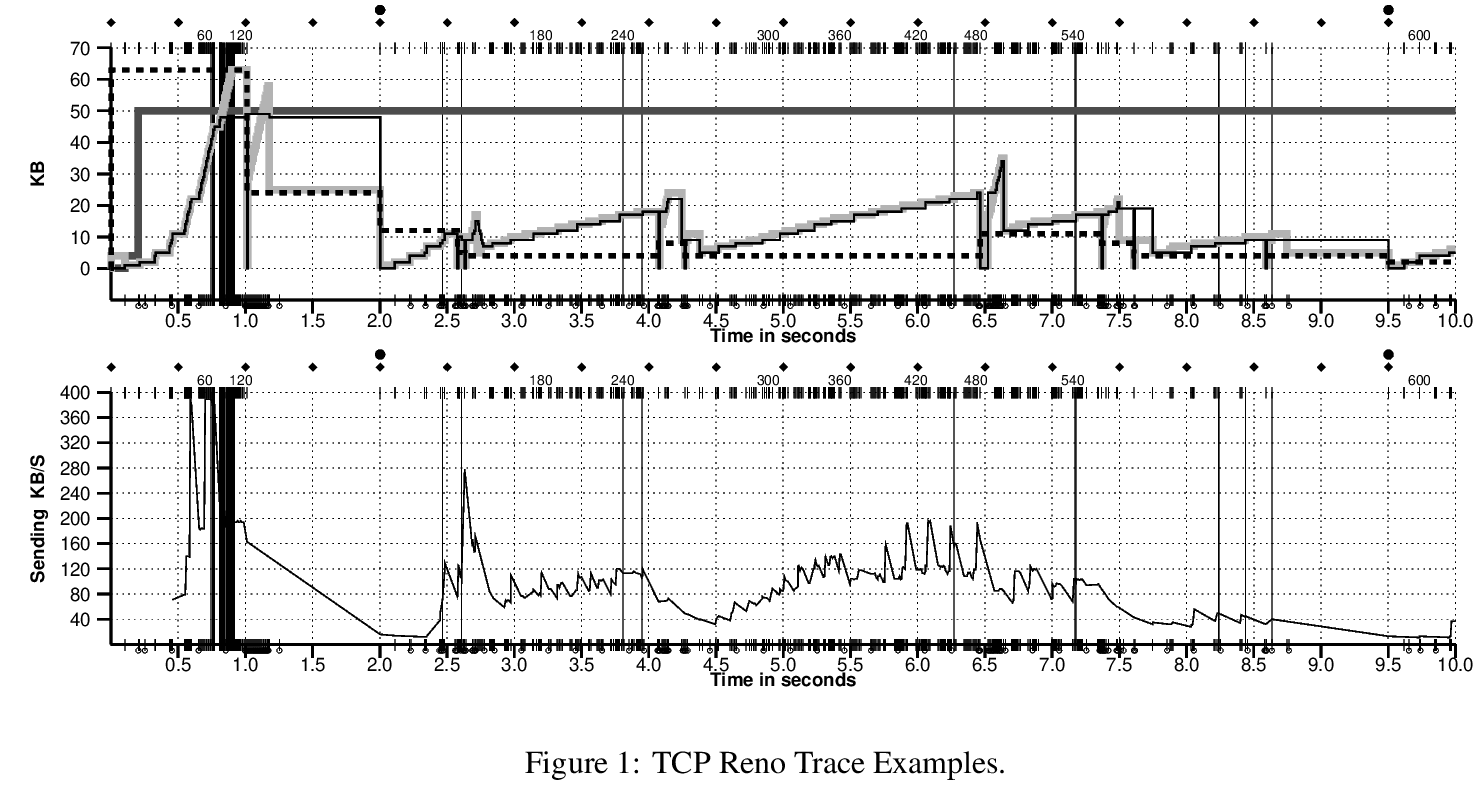
\includegraphics[width=0.9\textwidth]{../congest/vegas-fig1} \\
{
    \tiny from Brakmo, O'Malley, and Peterson, ``TCP Vegas: New techniques for
congestion detection and avoidance''} \\
    \small top thick, light-grey line = congestion window; dotted = slow start threshold
\end{frame}





\subsection{exercise: non-congestion losses} % FIXME: modify for decrease to 1
\begin{frame}{non-congestion losses}
    \begin{itemize}
    \item we were ignoring non-congestion losses
    \item suppose \myemph{1\%} loss rate from transmission errors
    \vspace{.5cm}
    \item 100 ms round trip time, very high bandwidth
    \item with TCP heuristics (+1 packet/RTT, half on loss)\ldots
    \item normal window size?
    \end{itemize}
\end{frame}



% FIXME: \subsection{exercise: convergence times}


